\newpage
\chapter{Tinjauan Pustaka} \label{Bab II}

\section{Tinjauan Pustaka} \label{II.Tinjauan}
Berisi penelitian terdahulu yang menjadi konsep / pendukung penelitian yang dilakukan. Lakukan pembahasan secara sistematis dengan menjelaskan masalah apa yang diangkat di penelitian terdahulu, metode yang digunakan, kontribusi yang diberikan, serta analisis penulis terkait dengan keunggulan atau keterbatasannya. Tuangkan perbandingan penelitian terdahulu dengan penelitian yang akan dikerjakan, minimal 5 jurnal pembanding (3 -4 tahun terakhir). Perujukan literatur dapat dilakukan dengan menambahkan entri baru di berkas \cite{knuth2001art}. \par

Kemudian penulis sebaiknya melakukan rangkuman terutama terkait dengan peluang pengembangan atau tugas akhir yang akan dilakukan \par

\begin{enumerate}
	\item Sistem Informasi Pendaftaran Haji dan Umroh Di PT Multazam Sriwijaya Barakah Palembang Menggunakan Metode Rapid Application Development. \blindtext
	\item Sistem Informasi Umroh Di PT XYZ Lampung Menggunakan Metode Rapid Application Development. \blindtext
\end{enumerate}

\begin{longtable}{| b{0.05\textwidth}|p{0.2\textwidth}|p{0.2\textwidth}|p{0.15\textwidth}|p{0.25\textwidth}|} % Longtable berguna agar tabel dapat terpotong di halaman baru
	\caption{Literasi Penelitian Terdahulu}
	\label{table:2.literasi}\\
	\hline
	No. & Judul & Masalah & Metode & Hasil \\
	\hline
	\endhead % Agar semua baris diatas ini diulang jika melewati halaman baru (repeat header row)
	1. & Sistem Informasi Pendaftaran Haji dan Umroh Di PT Multazam Sriwijaya Barakah Palembang Menggunakan Metode Rapid Application Development & Belum adanya sistem untuk pendaftaran haji \& umrah & Rapid Application Development & Sistem Informasi Pendaftaran Haji dan Umroh di PT Multazam Sriwijaya Barakah Palembang\\ 
	\hline
	2. & Sistem Informasi Umroh Di PT XYZ Lampung Menggunakan Metode Rapid Application Development & Belum adanya sistem untuk pendaftaran haji \& umrah & Rapid Application Development & Sistem Informasi Pendaftaran Umroh di PT XYZ Lampung\\ 
	\hline
	3. & Sistem Informasi Umroh Di PT XYZ Lampung Menggunakan Metode Rapid Application Development & Belum adanya sistem untuk pendaftaran haji \& umrah & Rapid Application Development & Sistem Informasi Pendaftaran Umroh di PT XYZ Lampung\\ 
	\hline
\end{longtable}

\section{Dasar Teori} \label{II.Teori}
Berisi teori / konsep yang berkaitan / digunakan dalam tugas akhir yang dikerjakan. Gunakanlah data melalui buku/jurnal referensi, publikasi tugas akhir, penelitian, buku, dan informasi web yang dapat dipertanggungjawabkan, hindari penggunaan dasar teori melalui tautan Wikipedia, surat kabar, atau portal berita, yang dapat memiliki isi yang tidak bersifat fakta. \par

Berikut adalah contoh penyisipan tabel menggunakan \verb|\begin{longtable}{}|: \par

\begin{longtable}{|c|c|c|c|}
	\caption{Contoh Tabel}
	\label{table:2.contoh}\\
	\hline
	Col1 & Col2 & Col2 & Col3 \\
	\hline
	\endhead
	1 & 6 & 87837 & 787 \\ 
	\hline
	2 & 7 & 78 & 5415 \\
	\hline
	3 & 545 & 778 & 7507 \\
	\hline
	4 & 545 & 18744 & 7560 \\
	\hline
	5 & 88 & 788 & 6344 \\
	\hline
\end{longtable}

\subsection{Subbab 1} \label{II.Subbab1}
Deskripsikan mengenai teori / konsep yang berkaitan / digunakan / menjadi acuan dalam penelitian. Kemudian berikan pembahasan sederhana mengenai penggunaannya di dalam tugas akhir yang Anda kerjakan. \par

Berikut adalah contoh penyisipan gambar menggunakan \verb|\begin{figure}[H]|:

\begin{figure}[H] % Kalau menggunakan H, posisi gambar akan tepat dibawah teks
    \centering
    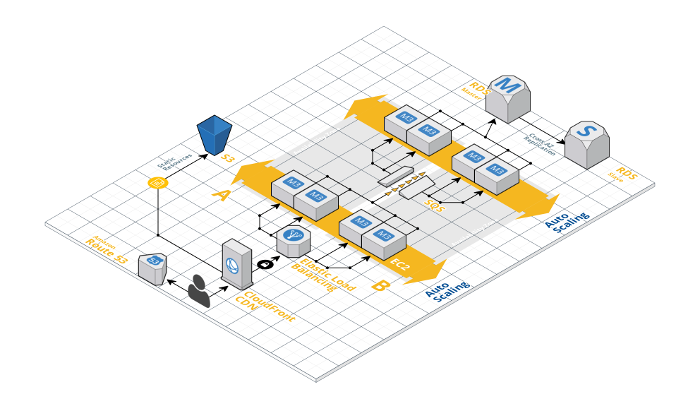
\includegraphics[width=0.8\textwidth]{figure/chapter-2-infrastructure-diagram.png}
    \caption{Contoh gambar}
    \label{fig:2.contoh}
\end{figure}

\subsubsection{Subsubbab} \label{II.Subsubbab1}

Berikut adalah contoh subsubbab. Ini adalah level subbab maksimal dalam laporan Tugas Akhir, dan tidak boleh lebih dalam.

\begin{figure}[H]
	\centering
	
\includegraphics[width=3cm]{figure/samplephoto.jpg}
	\caption{Contoh foto}
	\label{fig:2.foto}
\end{figure}

\subsection{Subbab 2} \label{II.Subbab2}
Untuk membuat sebuah persamaan, gunakan kode \verb|\begin{equation}| dibawah: \par

\begin{equation}
	x + 1 = 2
\end{equation}
\label{eq:2.sum}
\myequations{Fungsi x}

Berikut adalah contoh penulisan persamaan yang lebih kompleks, yaitu persamaan distribusi normal. \par

\begin{equation}
	P(x) = \frac{1}{{\sigma \sqrt {2\pi } }}e^{{{ - \left( {x - \mu } \right)^2 } \mathord{\left/ {\vphantom {{ - \left( {x - \mu } \right)^2 } {2\sigma ^2 }}} \right. \kern-\nulldelimiterspace} {2\sigma ^2 }}}
\end{equation}
\label{eq:2.normal}
\myequations{Distribusi normal}

Jika menuliskan banyak persamaan secara berurutan, gunakan  \verb|\begin{align}| atau \verb|\begin{gather}|: \par

\begin{align} 
	2x - 5y &=  8 \\ 
	3x + 9y &=  -12
\end{align}
\label{eq:2.SPL}
\myequations{Sistem persamaan linier}
